\subsection{Calibration} 

    \todoNow{add error analysis for the calib data}

    The calibration is needed to map each pixel on the CCD to a specific wavelength. Such a map is refered to as a wavelength solution. To do this, we need a light source with known frequencies, preferably many discret peaks. EXPRES uses a Thorium Argon lamp for an initial trial wavelength solution and a laser frequency comb (LFC) for an more precise solution.
    
    The Thorium Argon lamp produces 4,000 lines across 82 orders, which can be identified and mapped to a wavelength through a \emph{line atlas}. An intial wavelength solution for all pixels is then produced by linear interpolation. (I this project I have not done this calibration).

    The LFC generates a series of equadistant (evenly spaced) spectral lines, typically 20,000 lines across 50 orders. The range of the LFC is thus shorter, and for this reason the ThAr exposures can also be used for a rough calibration outside the LFC range. The frequencies of the LFC peaks are given by the relation
    
    \begin{equation}
        \label{eq:LFC_freq_eq}
        v_{n}=v_{\text{rep}} \times n+v_{\text{offset}}
    \end{equation}

    for integers $n$. The repetition rate $v_{\text {rep }}$ and offset frequency $v_{\text {offset }}$ are referenced against a GPS-disciplined quartz oscillator, providing calibration stability corresponding to a fractional uncertainty of less than $8 \times 10^{-12}$ for integration times greater than $1 \mathrm{~s}$. (p. 8, \cite{first_RV_from_EXPRES}). The values I have used in the calibration, $v_{\text{rep}} = 14e9$ and $v_{\text{offset}} = 6.19e9$, were provided by Lars Buchhave, but may be outdated. 

    The location of the LFC peaks (also refered to as modes) I determine first with a peak finding algorithm from scipy and then by fitting a super-gauss with a linear background to each peak:
    
    \begin{equation}
        \label{eq:LFC_super_gauss}
        A \exp \left(-\left(\frac{\left(x-\mu\right)^{2}}{2 \sigma_{x}^{2}}\right)^{P}\right) + B(x-\mu) + C
    \end{equation}
    
    A super-gauss is a regular gaussian but with an extra parameter, here denoted $P$, that allows the top of the peak to be flattened. To map the LFC peaks with the frequencies given by equation (\ref{eq:LFC_freq_eq})

    I can then use the intial wavelength solution (provided in the data that I have used) to map the LFC peaks to the frequencies given by equation (\ref{eq:LFC_freq_eq}). 

    From here, I have explored two approaches to produce a wavelength solution for all pixels: cubic interpolation and polynomial fit. I can evaluate the quality of the interpolation calibration by choosing to omit every second peak from the interpolation and then computing the residuals between the omitted peaks and the resulting interpolation function. For the polynomial, I can compute residuals simply by subtracting the location peaks from the fit function. Residuals from the two methods are compared in figure \ref{fig:calib_poly_vs_interp}.

    \begin{figure}[ht]
        \centering
        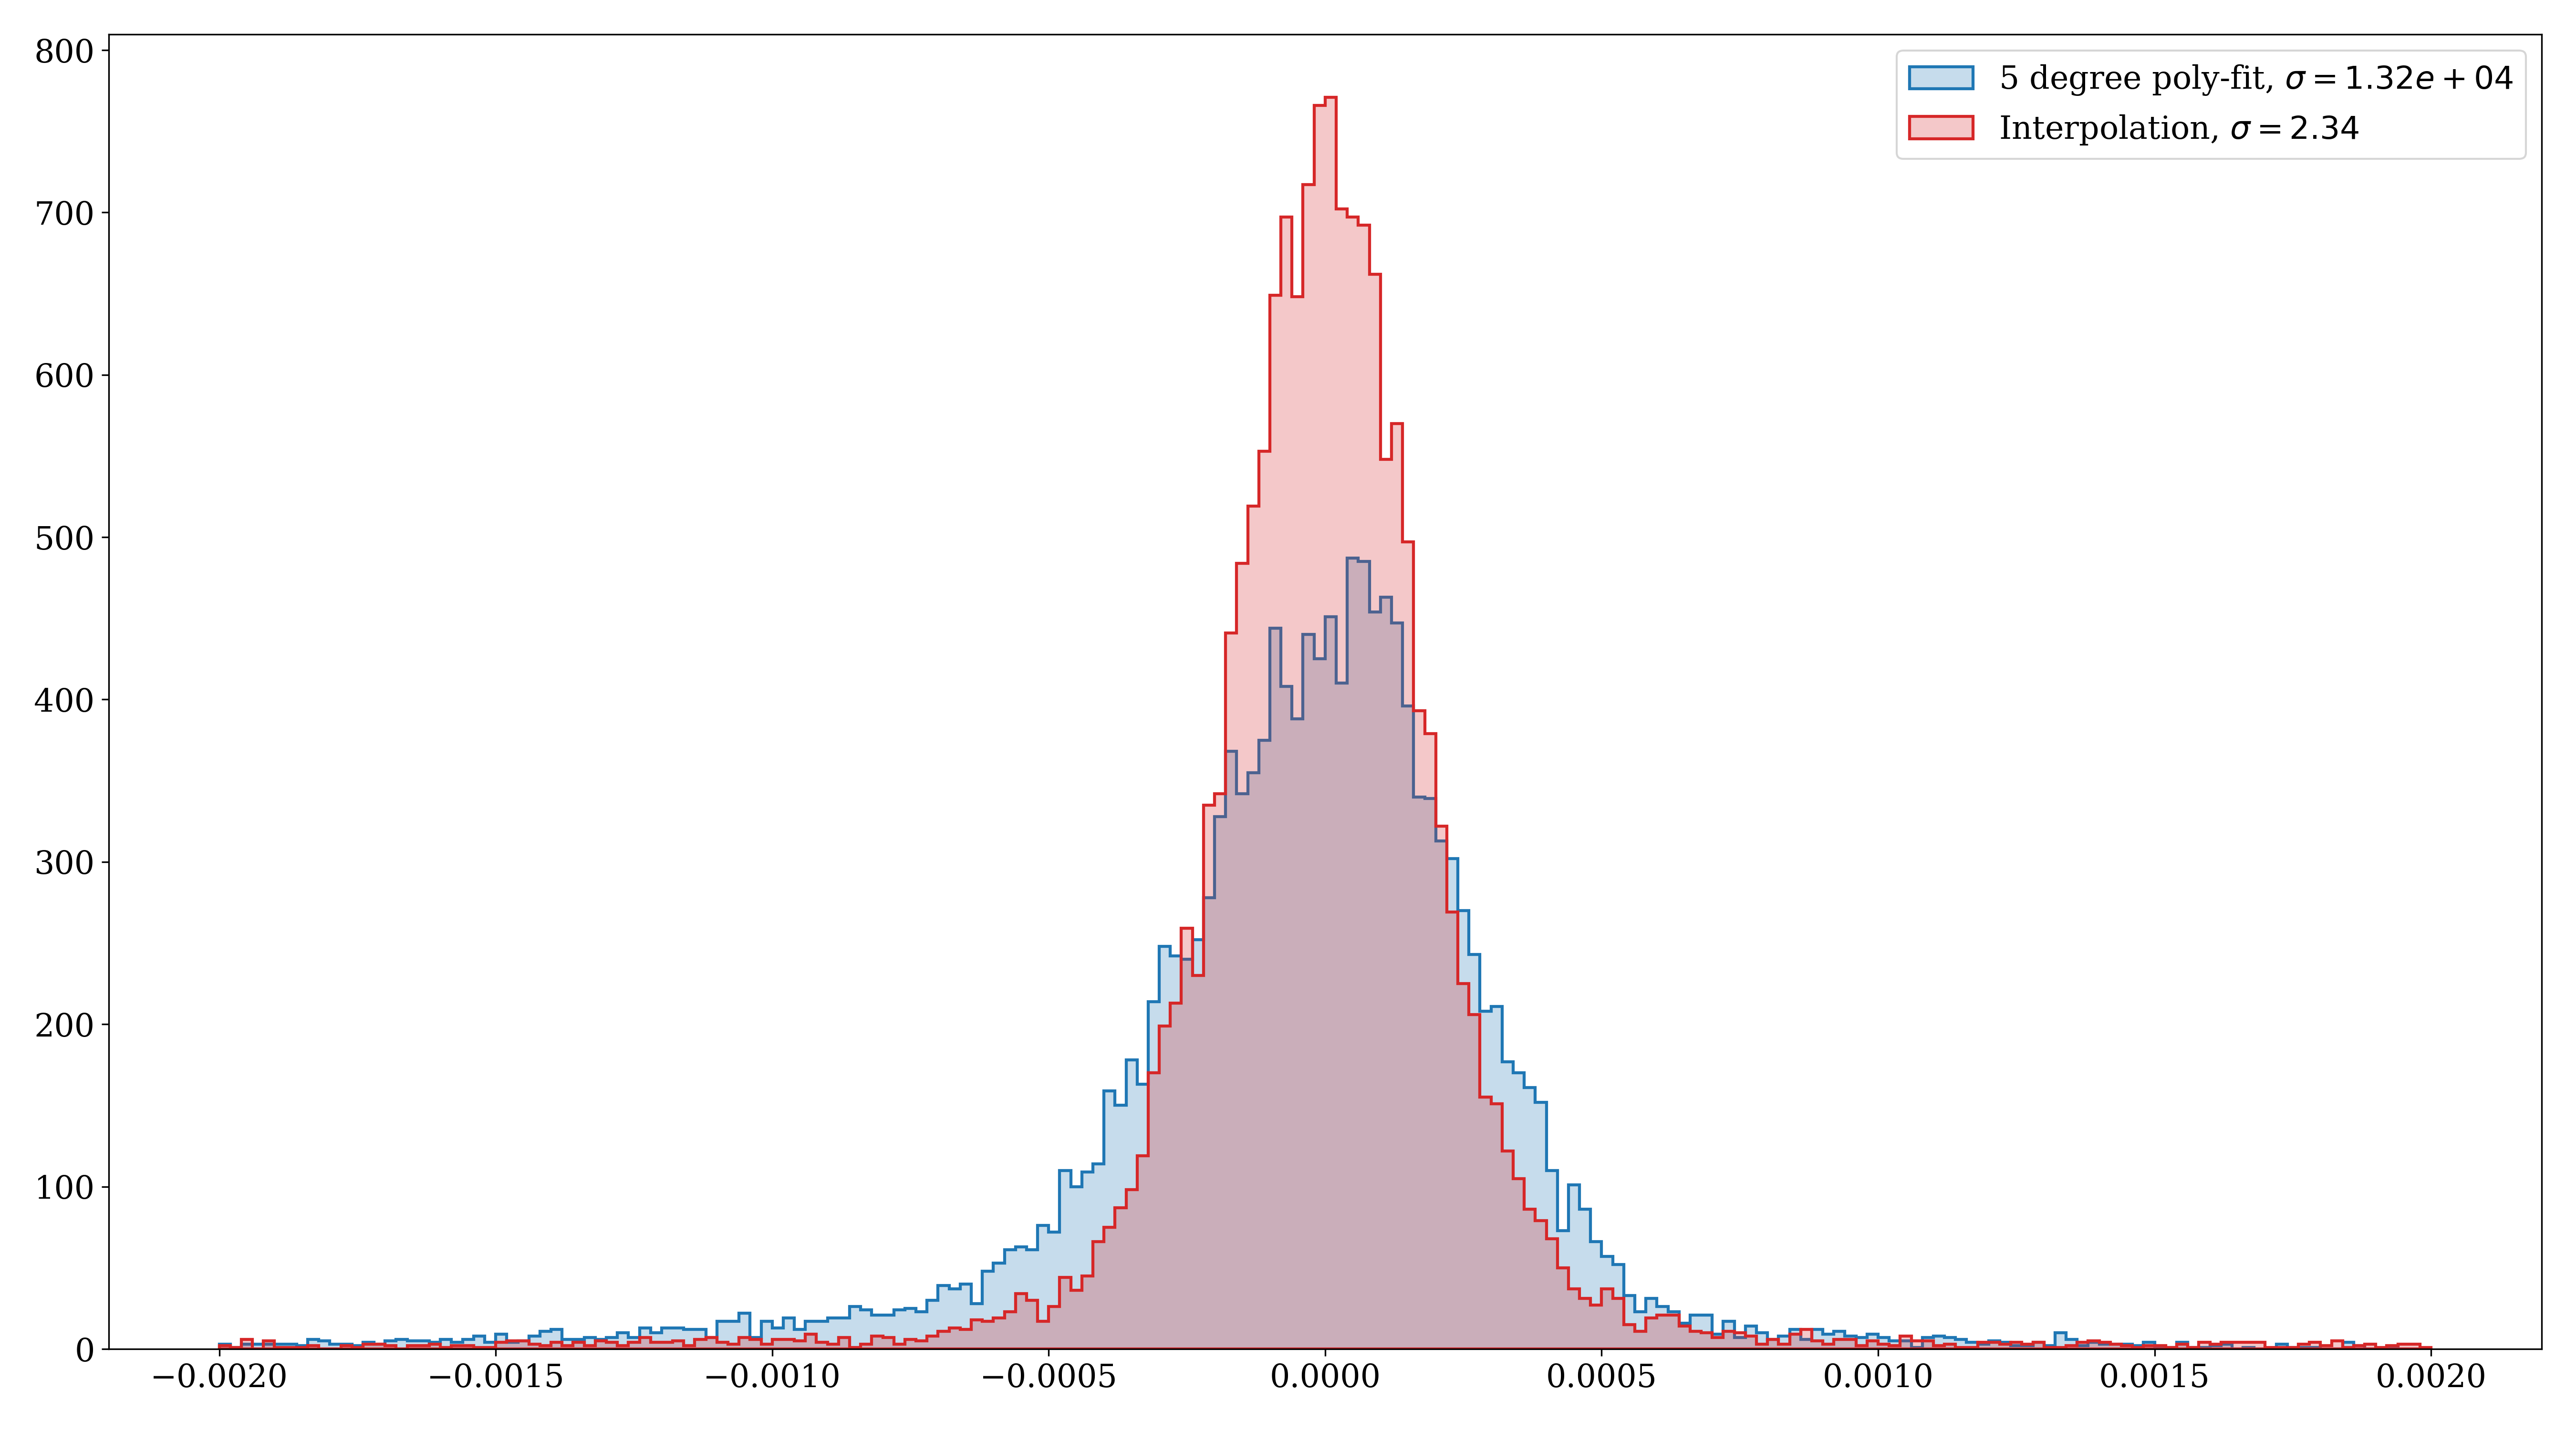
\includegraphics[scale=0.40]{figures/hist_peak_residuals_poly_and_interp.png}
        \caption{Residuals from calibrations performed through poly-fit and interpolation. Both results contain approximately the same amount of points, but the poly-fit has a much larger spread and therefore appears smaller. \todo{polyfit has 18373 lines, interp has 16888. Why? } \todo{find out x units}}
        \label{fig:calib_poly_vs_interp}
    \end{figure}

    The standard deviation of the residuals from the interpolation come out much smaller than that of the polyfit (values specified in figure \ref{fig:calib_poly_vs_interp}), in this example, suggesting that the interpolation method is superior. It is also worth noting that because the interpolation was done on only half the data points, it will be even better when performed on all data points. A similar comparison was done to determine that the polynomial fit got better with increasing degrees until 5th. \todo{specify what file?}

    \vspace{0.5cm}

    \todo{add graph comparing residuals using gauss vs super gauss}

    \todo{perhaps add plot of changes in parameters across the CCD}

    \todo{specify run times for calibration using poly fit and interp}

    \subsubsection{Errors in the calibration data}

    \todoNow{Rewrite this:}

    The chi2 values should be equal to the number of parameters in the fit. We have 5 parameters (although Troels said something about 12 or 14 .... why?). So we can see that the initial errors give a chi2 distribution that is waaay to flat. If we multiply by $\sqrt{3}$ we get something better. $\sqrt{10}$ looks perhaps even better! But, the p-value distribution should be flat (TODO: ask Troels why or look it up), so we can see that the original errors are probably too small and the ones multiplied by $\sqrt{10}$ are too high, because we get a spike at 1 — i.e. the fit is too good. The spike at 0 is okay, those are just all the fits that sucked and should perhaps be removed. 

    The Chi2 values are about a factor 3 too larger, thus the uncertainties are about a factor sqrt(3) too small. My evaluation is based on the notion, that the Prob-distribution should be about flat, when it is right (with peaks at the ends). We then seem to have a good fraction (10%?), which are poor fits, perhaps to be considered either for omission or increased uncertainty.

    With this correction the standard deviation of the residuals of the interpolation decreases from 2.34 to 0.934.

    \begin{figure}[ht]
        \centering
        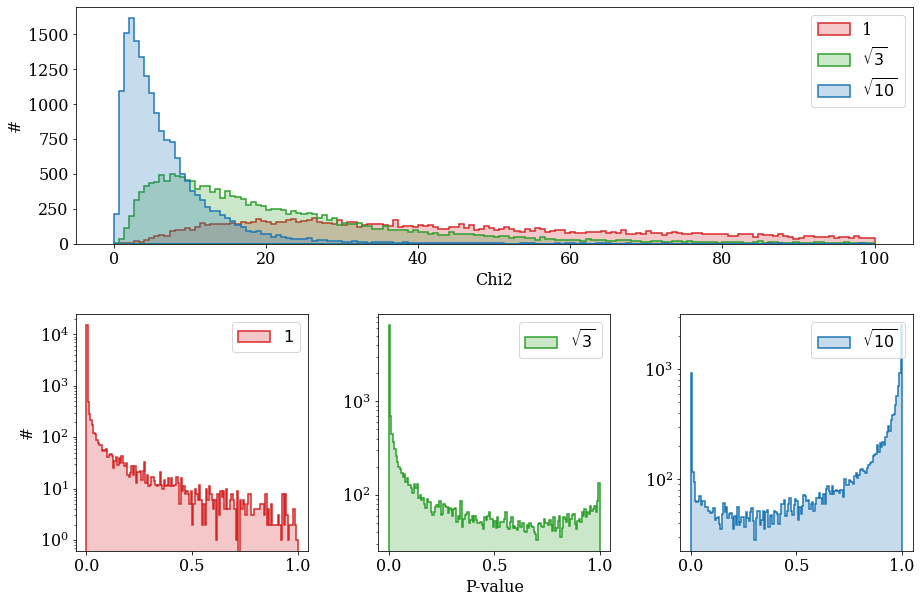
\includegraphics[scale=0.40]{figures/calib_errors.png}
        \caption{Chi2-values and P-values from individual LFC peak super-gauss fits with photon count (spectrum) errors multiplied by different scale-factors (1, $\sqrt{3}$ and $\sqrt{10}$). As the distribution of P-values generally should be flat, the graphs suggest that the given errors (scale-factor 1) are too small. Multiplying errors by $\sqrt{3}$ is a conservative correction.}
        \label{fig:calib_errors}
    \end{figure}


    \todo{Check the resulting sigma for different error scale factors}


\subsection{RV extraction}





    \begin{itemize}
        \item Hist fit / cross-correlation
        \begin{itemize}
            \item Order approach
            \item Feature approach
            \item (Run times)
        \end{itemize}
        \item Extracting relative radial velocities from over constraint system (Matrix reduction to circumvent correlations)
        \item Future ideas
        \begin{itemize}
            \item Auto encoder
        \end{itemize}
    \end{itemize}

